%%%%%%%%%%%%%%%%%%%%%%% file template.tex %%%%%%%%%%%%%%%%%%%%%%%%%
%
% This is a template file for Web of Conferences Journal
%
% Copy it to a new file with a new name and use it as the basis
% for your article
%
%%%%%%%%%%%%%%%%%%%%%%%%%% EDP Science %%%%%%%%%%%%%%%%%%%%%%%%%%%%
%
%%%\documentclass[option]{webofc}
%%% "twocolumn" for typesetting an article in two columns format (default one column)
%
\documentclass{webofc}
\usepackage[varg]{txfonts}   % Web of Conferences font
%
% Put here some packages required or/and some personnal commands
%
%
\begin{document}
%
\title{Extending ROOT through Modules}
%
% subtitle is optionnal
%
%%%\subtitle{Do you have a subtitle?\\ If so, write it here}

\author{\firstname{Brian Paul} \lastname{Bockelman}\inst{1}\fnsep\thanks{\email{bbockelm@cse.unl.edu}} \and
        \firstname{Oksana} \lastname{Shadura}\inst{1}\fnsep\thanks{\email{oksana.shadura@cern.ch}} \and
        \firstname{Vassil} \lastname{Vassilev}\inst{2}\fnsep\thanks{\email{vasil.georgiev.vasilev@cern.ch}}
        % etc.
}

\institute{University of Nebraska Lincoln, 1400 R St, Lincoln, NE 68588, United States
\and
           Princeton University, Princeton, New Jersey 08544, United States
          }

\abstract{%
The ROOT software framework is foundational for the HEP ecosystem, providing capabilities such as IO, a C++ interpreter, GUI, and math libraries. It uses object-oriented concepts and build-time modules to layer between components. We believe additional layering formalisms will benefit ROOT and its users.

We present the modularization strategy for ROOT which aims to formalize the description of existing source modules, making available the dependencies and other metadata externally from the build system, and allow post-install additions of functionality in the runtime environment. Modules can then be grouped into packages, installable from external repositories to deliver post-install step of missing packages. This provides a mechanism for the wider software ecosystem to interact with a minimalistic install. Reducing intra-module dependencies improves maintainability and code hygiene. We believe helping maintain the smallest “base install” possible will help embedding use cases.

The modularization effort draws inspiration from the Java, Python, and Swift ecosystems. Keeping aligned with the modern C++, this strategy relies on forthcoming features such as C++ modules. We hope formalizing the module layer will provide simpler ROOT installs, improve extensibility, and decrease the complexity of embedding in other ecosystems.
}
%
\maketitle
%
\section{Introduction}

One clear advantage of object-oriented systems is the ability to have abstraction layers provide separation between the user of an object and the implementer.  Ultimately, this helps projects scale to very large code bases.  Another technique for scaling projects is using modularization: grouping together significant functionality into distinct units with clear points of interaction.  While ROOT has a strong history in object-oriented programming, it doesn’t have a strong concept of modules.  Thus, we propose to add four concepts to the ROOT ecosystem:
\begin{enumerate}
\item Module: A set of interdependent classes implementing coherent functionality and providing well-defined APIs.
\item Library: a module or set of modules  which makes sense to be together and that can be used in a program or another library.
\item Package: A distinct, self-describing resource (file, URL) that provide one or more modules.
\item Package database: A record of all packages currently available in a ROOT installation.
\item Package manager: An actor that can locate and install packages into a ROOT installation from a package reference, along with their transitive dependencies.
\end{enumerate}
There exist other legacy large object-oriented software systems  which, similar to ROOT, consisting of a large number of interdependent  and loosely-coupled classes, mostly organized as set of libraries and build targets.  Classes are often the lowest level of granularity to serve as a unit of software modularization. In ecosystems such as Java,  Python and C++, a further package structure can allow software developers organize their programs into components. A good organization of classes into identifiable and collaborating packages eases the understanding, maintenance of software. To improve the quality of software modularization, assessing the package organization is required.

Since we address large software systems as ROOT framework, consisting of a very large number of classes and packages, we consider that packages are the units of software modularization. 

Packages and modules are not synonymous concepts.  A module is a set of functions, types, classes and etc., defined in a common namespace. We can define module also as a set of related functionality that exposes a well-defined API. A library is a module or set of modules  which makes sense to be together and that can be used in a program or another library. A package is a unit of distribution that can contain a library or an executable or both. Considering a library is a set of modules, a package bundles a set of modules with related metadata (such as name, version and dependencies) which can be distributed as a standalone unit.

\section{Motivation}

Modularization defines a way of grouping of functionality from a software product. It outlines groups in form of modules which identify a particular piece of functionality to solve a set of problems. In general, modularization helps reducing management, coordination and development costs.
We aim to define a set of mechanisms that enables a modular version of ROOT, centered around C++ modules, working as package-centric ecosystem.

Library dependencies alone result in an imposingly complex relationship diagram. By introducing a module layer, we would provide better boundaries between components, allowing ROOT to scale as a project. For example, the level of expertise for the contributor needs can be more localized. It could means for project, that ROOT by itself could evolve in new phase, and can potentially interact with many more packages and while turn itself into even more useful toolkit. 

By making the boundaries and relationships more explicit through modules, we can better define and implement a “minimal ROOT,” increasing the chances its functionality can be embedded in other contexts.  This enables ROOT users to interact with the wider data science ecosystem.

Packages and package management provide a mechanism for ROOT users to socialize and and reuse projects built in the context of ROOT, it helps to make ROOT more flexible and open for new customers.  This allows ROOT to continue to serve as a community nexus.

In particular, this provides the ROOT team with an improved mechanism to say “no” to new modules within the ROOT source itself as users can simply share their packages among each other or in a common store such as github.

\section{ROOT components and packages}

ROOT code is organized into a set of logical sub-directories, except of Core library, that has more complex structure of subfolders. In this case, each of directories can be roughly thought of as a module. 

A module is a single unit of code distribution (set of classes) for a framework or an application that is built and shipped and that can be imported by another module with a hook (such as  include or an import keyword). A program may have all of its code in a single module (or inside of more modules), or it may import other modules as dependencies.

This model requires a few definitions:
\begin{enumerate}
\item Define modules as a ROOT “component”. It could be also defined as a module or package with single module inside which is distributed and maintained through 'standard' ROOT (i.e. lives in root.git).

For example, we could define a ROOT module as a subsystem for numerical minimization (Fumili or Minuit(2)), that is required to complete function of search of extreme points or is intended to be included as a part of a finished, packaged, and labeled package for one-dimensional and multidimensional minimization to provide full minimization functionality for ROOT ecosystem.

Figure 1 shows possibility to combine any type custom package based on user required components, like for example hypothetic ROOT-ML package that consists of TMVA and RDataframe module with its dependencies.

\item Every facility is provided by exactly one module.
\end{enumerate}

Taking in account ongoing work on C++ modules in ROOT, we could try to align work together with ROOT modularization efforts. On one hand, C++ modules provide an simple way to use software libraries that provides better compile-time scalability and eliminates problems to access the API of a library. They improve encapsulation and outline a well-defined relationship between public and private part of the code split into an implementation and interface. On the other hand, modules have a weak side in versioning and binary distribution of modules among others problems.

\begin{figure}
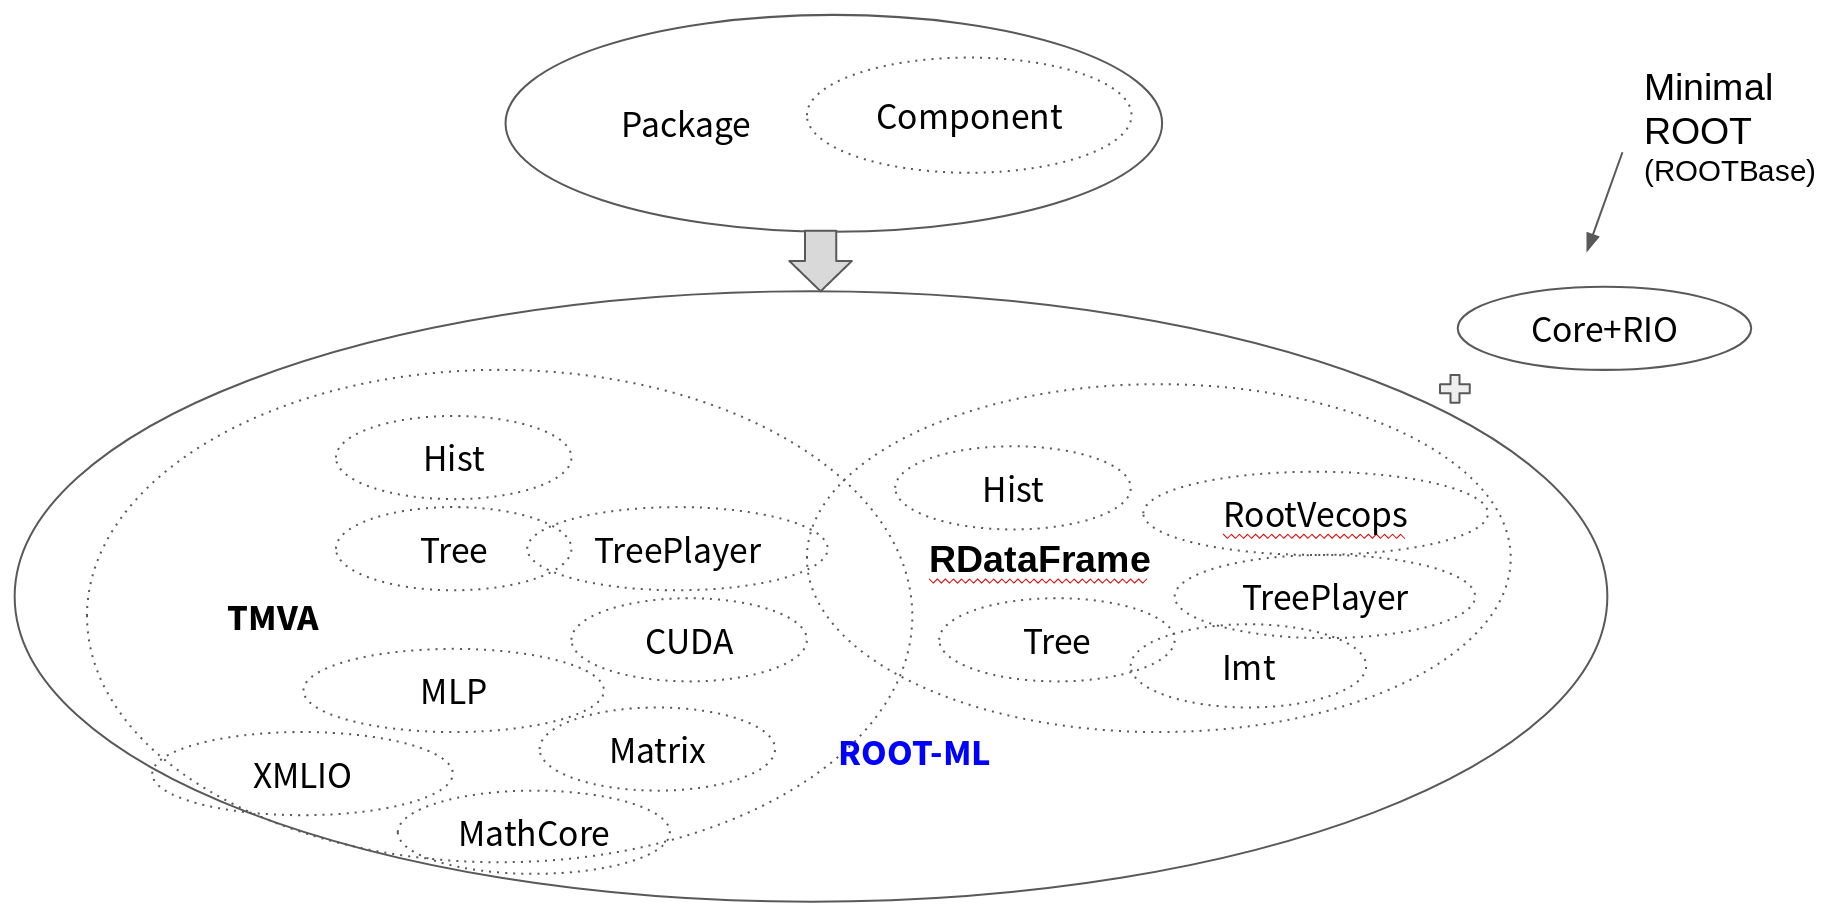
\includegraphics[width=1.0\linewidth]{picture/1.png}
\caption{Example of ROOT component and package.}
\label{interp}
\end{figure}

\end{enumerate}

ROOT package is defined as a grouping of software for data analysis and associated resources, intended for it distribution (extension or upgrade of  ROOT functionality). 
The definition of package assumes a contract for code organization in order to simplify the build and deploy steps. The contract defines a manifest file and particular organization of each module.

Manifest file is a file which describes the content of a package. It has self-describing and easy to process by machines format. The manifest file contains information about how the contents should be built, deployed and versionized.

Package byproducts are a set of modules, which could be packed as a library and/or executable, with documentation and unit tests.

One of simple case of ROOT package is  ROOT Base, which include Cling, IO and Core modules. This is our fundamental part from which we start to build a ROOT.
Other example of ROOT package is abstract “Math” package, that could consist of multiple math related modules depending on package vendor.
To have a successful socialization of ROOT project via modularization, we need to agree on a format of ROOT package and define set of available modules and its packages for existing monolithic ROOT framework (e.g. manifest example was inspired by Swift manifests and should be written in YAML).

To provide motivation for introducing manifest files, we will to try to list its use-case scenarios:
\begin{enumerate}
\item Situation when we need to deal with ROOT subsystem user or developer (e.g. io). The manifest file is generated by the info in the build system.
\item Situation when we need to deal with third party developer (PhD student) who has some amount of files and does not know anything about build systems and  would like to describe in a human form what package does and what ROOT components it depends on.
\item Situation when we need to deal with experiment librarian that knows exactly what he need - writing manifest file or some other configuration to tell ROOT what packages he need for the ideal scenario. The other scenario could be to describe a pre-built package.
\item Situation when we need to deal with member of physics group that want to have particular library to be auto-build on demand or to socialize his own library.
\end{enumerate}

%\begin{figure}
%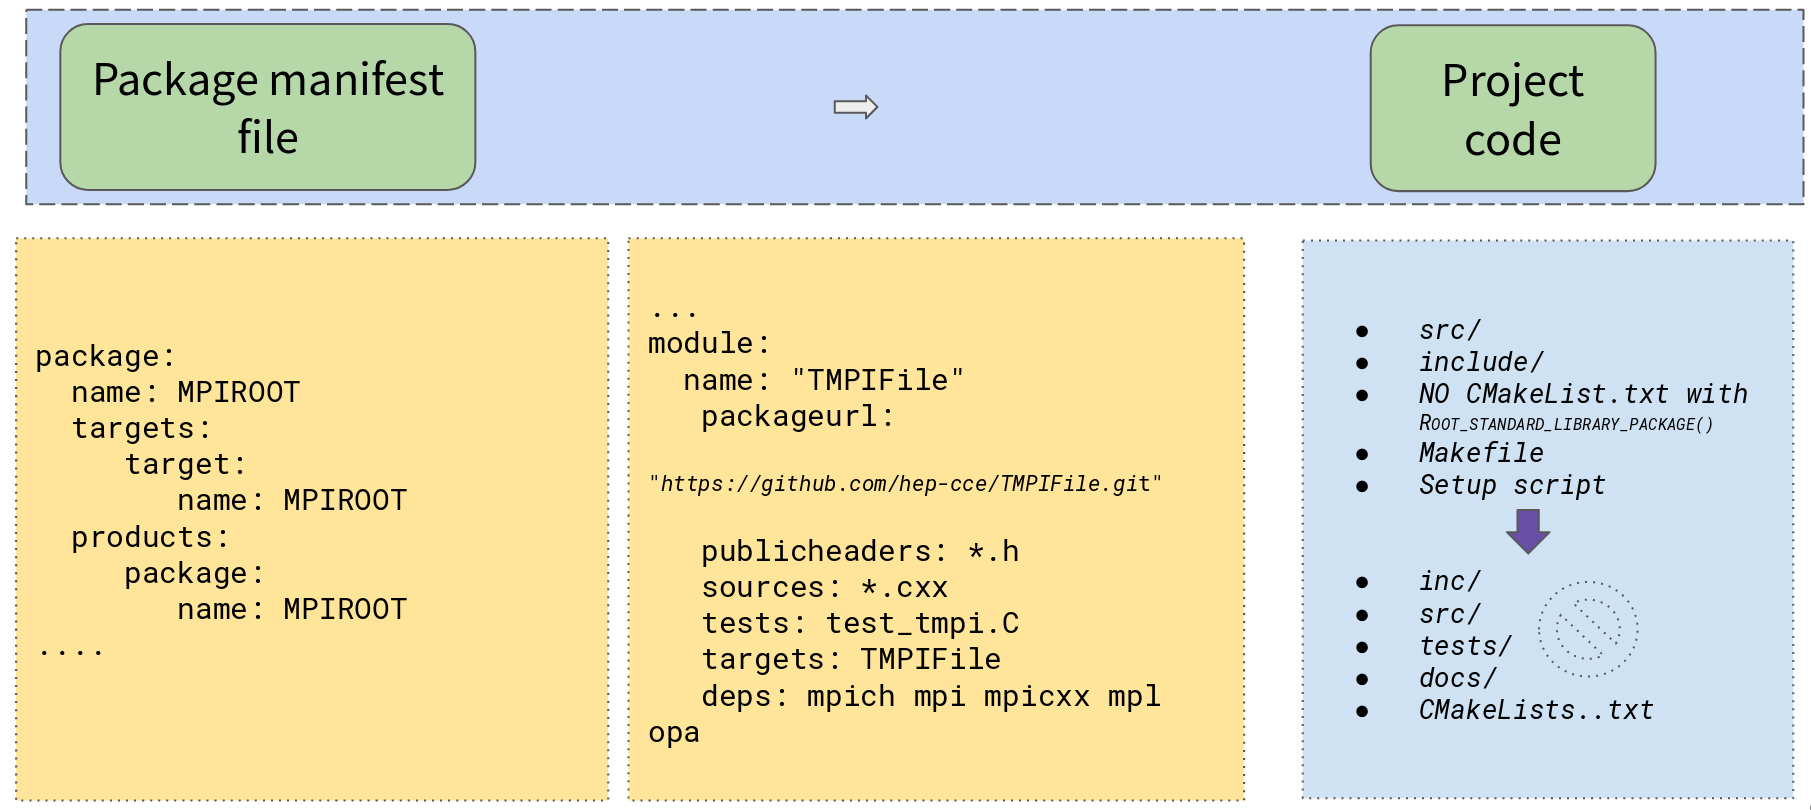
\includegraphics[width=1.0\linewidth]{picture/2.png}
%\caption{}
%\label{interp}
%\end{figure}

%\begin{figure}
%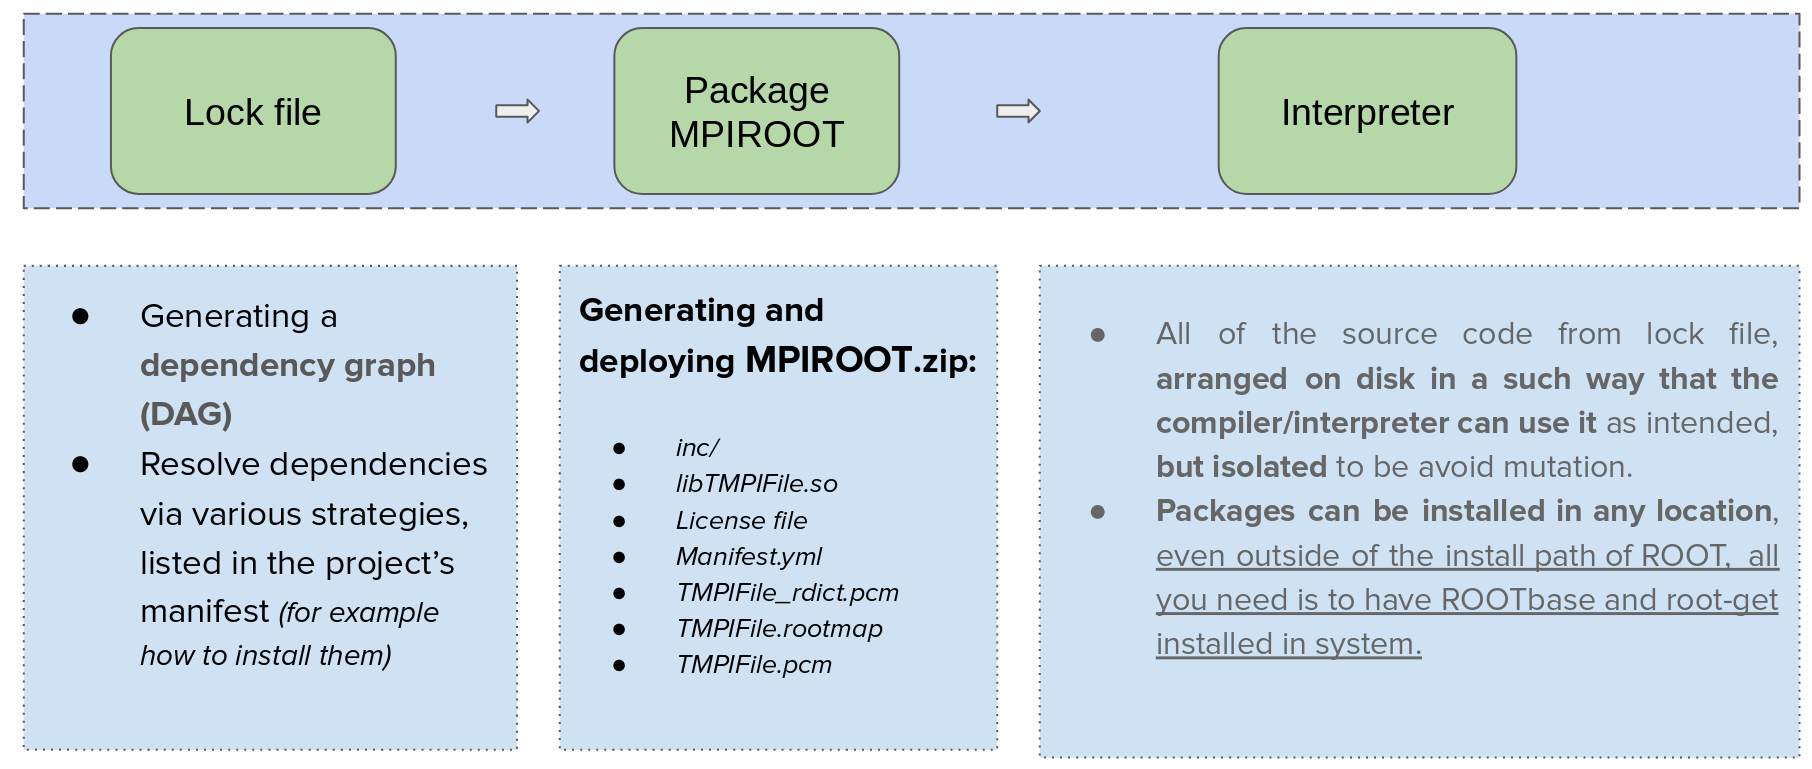
\includegraphics[width=1.0\linewidth]{picture/4.png}
%\caption{}
%\label{interp}
%\end{figure}

\section{ROOT Package Manager and "lazy install" method}

Package manager is a tool (usually a standalone tool) for managing the distribution of software code. 
Here in this article we will try to focus on two interesting for us entities from package manager classification (third one is OS package manager (OSPM) that we are not interested in current discussion):
\begin{enumerate}
\item Language package manager (LPM): an interactive tool (e.g., `go get`) that can retrieve and build specified packages of source code for a particular language.
\item Project/application dependency manager (PDM): an interactive system for managing the source code dependencies of a single project in a particular language. That means specifying, retrieving, updating, arranging on disk, and removing sets of dependent source code, in such a way that collective coherency is maintained beyond the termination of any single command. Its output — which is precisely reproducible — is a self-contained source tree that acts as the input to a compiler or interpreter. You might think of it as “compiler, phase zero.”
\end{enumerate}
We think about ROOT package manager as a mix of LPM and PDM, since ROOT has incorporated c++ interpreter in its code source.

A ROOT package managing system can manage the package lifetime to ensure sustainability in a transparent to the user way. The role of the ROOT package manager is to reduce coordination costs by automating the process of downloading and building all of the dependencies for a project required for users, experiments or total community.

One of main challenges is to define package granularity. The best strategy is to left this decision for the users. Packages should not contain too little and too big modules because this in a way defeats the purpose of modularization. In the same time packages should not contain too many and too small modules because this introduces a lot of package management overhead.

When a project's packages have requirements that conflict with one another, it creates a situation defined as "dependency hell". Dependency hell is a common problem found in software that are built using an add-on software package or that rely on one for complete functionality. Dependency hell can take many forms and occur for many reasons, such as the need to install add-on software libraries, the need for long chains of installations, problems with a conflicting program, the creation of circular dependencies and more.
Often, rather than "reinventing the wheel", software should be designed to take advantage of other software components that are already available, or have already been designed and implemented for use elsewhere.

Definition of package engine is based on next set of operations executes the commands and macros in the preparation section of the manifest file, checks the contents of the manifest, executes the commands and macros.

On current stage of research, it is really important  to define minimal requirements, definition and format of a module, package and manifest file. Our goal is to proceed ahead with a problem of modularization and separability of Core part and other various functionality of ROOT. It gives to users more flexibility and possibility to combine various feature builds without rebuilding whole ROOT from beginning. Separation of code on modules and packages could allow to have  a way easily to associate functionality with a component you would like to use in ROOT.

Minimal requirement for ROOT package manager is  to be able to define the dependency and its version, and it could be done in manifest of package. It could be done either for ROOT packages or for external dependencies (compression algorithms packages for example). This should be a basic schema for distribution packages that are stored in  https://github.com/ and defined as dependencies.
Maximum requirements for package manager could be a next set of features (the list is inspired by functionality of Swift Package Manager, which is supported by a large Swift community):
\begin{enumerate}
\item Automated testing
\item Cross-platform packages
\item Support for other build systems (homebrew and etc.)
\item Support for version control systems
\item Library-based architecture
\item Standardized licensing (it is a complex problem for CMS experiment, for example)
\item A package index
\item Importing dependencies by source URL
\item Module inter-dependency determination
\item Dependency resolution
\item Resource management.
\end{enumerate}

Important part of design is usage of Clang C++ modules technology, that are the precompiled headers that can optimize header parsing, providing loading on-demand code from C++ modules. It is similar to ROOT precompiled header (PCH), but more separable and modular. ROOT runtime C++ modules will solve problem that ROOT PCH can be only single in the system: it is important feature for ROOT PM design. In the same time while using C++ modules for PM, we will try to help to solve a global problem of distribution C++ modules.
 
Reusing concepts from introduction C++ module infrastructure for ROOT, we can try to follow the ideas of Swift Package Manager and implement a standalone tool for ROOT modularization. ROOT team is working on enabling C++ modules and runtime C++ modules for 6.16 release.

\section{Evolving “ROOT Minimal” to “ROOT Base”}

While using CMake generation of libraries dependency graph, we can easily notice, that it is extremely hard to define “heart” part of ROOT. We need to start to work on modularization of ROOT package from the bottom to the top, trying to to build new ROOT modular system step by step.

ROOT’s build system provides a “minimal ROOT” option that suppose to deliver basic or essential functionality of ROOT, required for basic I/O and data analysis operations.
After evaluation of components built when this option is enabled, we believe that “ROOT Minimal” has migrated away from its original goal of a “core-like” ROOT; we aim to trim it down and to what we will consider the “base module” in this proposal.
Our plan is to start with three components:
\begin{enumerate}
\item Core
\item RIO
\item Cling.
\end{enumerate}

We will form ROOT base by taking these three modules and their transitive dependencies using CMake-based introspection.

TCling, an interpreter interface in ROOT, can help to provide an API, to contribute a set of operations with interpreter, including generation of the dictionary for the C++ classes, allowing operations with mangled names for a method of a class and etc.
After reviewing functionality of interpreter interface, we can define future handles for modularization project:
\begin{enumerate}
\item GetClassSharedLibs("ClassName") method gets the list of shared libraries containing the code for class "ClassName" and enable usage of “-I” option to be able to search custom includes, that are not in the rootmap;
\item AddIncludePath() method given path to the list of directories in which the interpreter looks for include files and load library containing the specified class.
\end{enumerate}

Other problem is how to connect the PM to ROOT interpreter. This is where CMake falls short as it does not have any support for steps happening after build/install time PM allows bootstrapping minimal ROOT and installing packages automatically on demand. It provides a basic interpreter functionality,  which will allow to install on demand ROOT components and use them directly in the same session.

\section{root-get prototype}

We provide a tool that help to provide dependency management or "lazy-install" package management system for ROOT (Figure 2). It consists of multiple modules that provide various functionality for package management:
\begin{enumerate}
\item Analyzer - analyzing routines for package management environment, that are checking operation system environment and available packages.
\item Generator - generator of manifests for ROOT or checking procedure for provided manifests for external packages.
\item Downloader - routines helping to download packages from github or other sources.
\item Resolver - package management database generation module and resolution of dependencies via direct acyclic graph.
\item Builder - building package scripts.
\item Intergrator - installation and deployment routine for package. 
\end{enumerate}

\begin{figure}
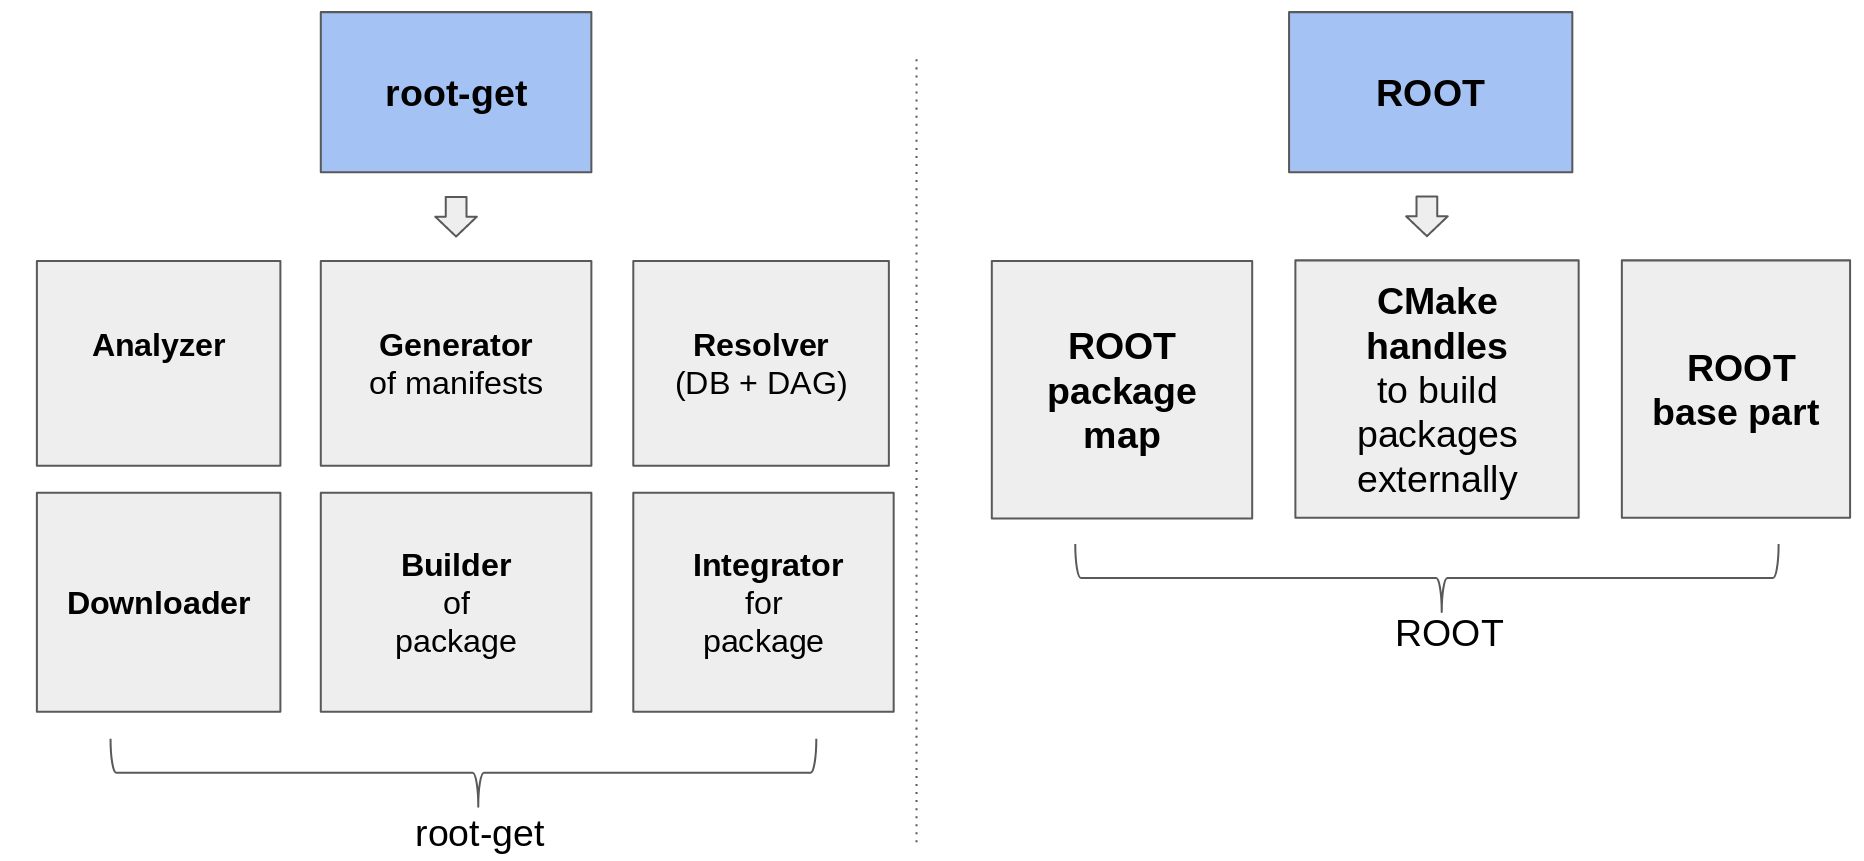
\includegraphics[width=1.0\linewidth]{picture/3.png}
\caption{ROOT "lazy-install" components.}
\label{interp}
\end{figure}

\section{Conclusions}

In these article we described package management ecosystem for ROOT. We defined a minimal and full set of requirements requirement for ROOT package manager. All ideas was adopted in a preliminary prototype that can download and install packages. A prototype can be connected to ROOT runtime and serve as a runtime dependency management tool.

\section{Acknowledgment}

%
% BibTeX or Biber users please use (the style is already called in the class, ensure that the "woc.bst" style is in your local directory)
% \bibliography{name or your bibliography database}
%
% Non-BibTeX users please use
%
\begin{thebibliography}{}
%
% and use \bibitem to create references.

\bibitem{root}
Rene Brun and Fons Rademakers, ROOT - An Object Oriented Data Analysis Framework, Proceedings AIHENP'96 Workshop, Lausanne, Sep. 1996, Nucl. Inst. and Meth. in Phys. Res. A 389 (1997) 81-86.
%
\bibitem{rootcxxmodules}
% Format for Journal Reference
Vassilev, Vassil. (2016). Optimizing ROOT's Performance Using C++ Modules. Journal of Physics: Conference Series. 898. . 10.1088/1742-6596/898/7/072023.

% Format for books
\bibitem{cxxmodules}
Clang C++ Modules, https://clang.llvm.org/docs/Modules.html


% etc
\end{thebibliography}

\end{document}

% end of file template.tex

<div id='footer'><table width='100%'><tr><td class='right'><a href='http://fusioninventory.org/'><span class='copyright'>FusionInventory 9.1+1.0 | copyleft <img src='/glpi/plugins/fusioninventory/pics/copyleft.png'/>  2010-2016 by FusionInventory Team</span></a></td></tr></table></div>